\section{Le CERN}\label{chapter-LHC-section-CERN}
%Les origines du CERN remontent aux années 1940
%Un petit groupe de scientifiques visionnaires d'Europe et d'Amérique du Nord estiment nécessaire que l'Europe dispose d'une infrastructure de recherche en physique de calibre mondial. Il s'agit d'endiguer la fuite des cerveaux vers l'Amérique, qui avait commencé durant la Deuxième Guerre mondiale, et d'offrir un moyen d’unifier l'Europe d'après-guerre.

\begin{figure}[h]
\centering
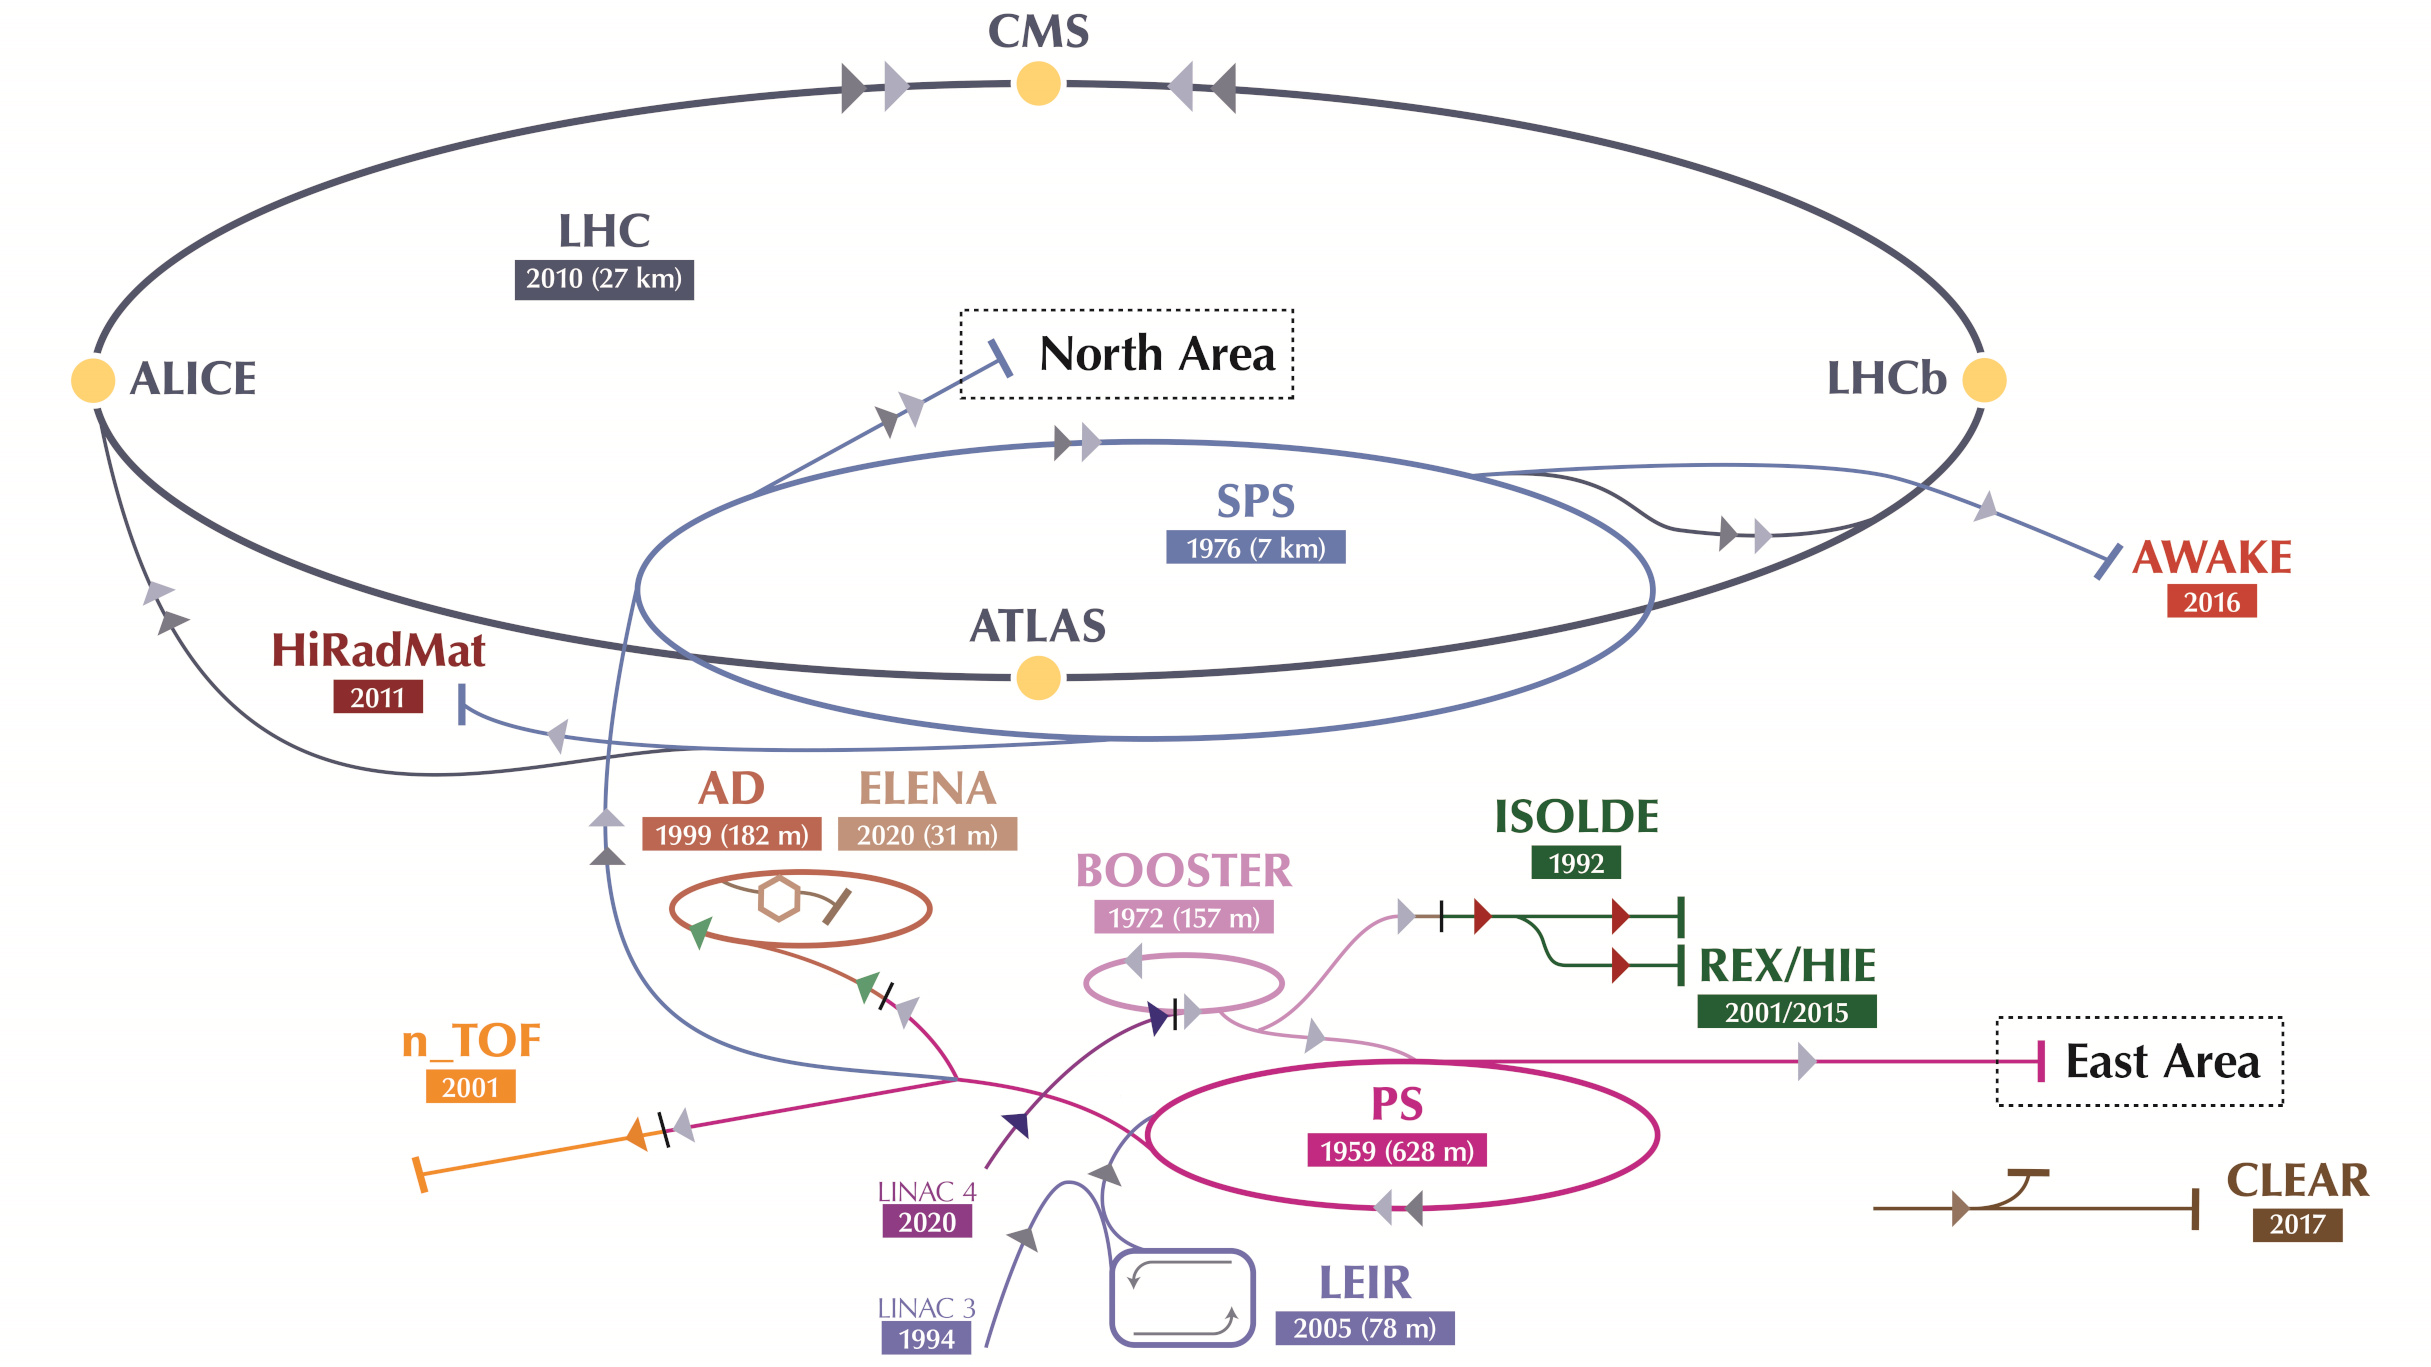
\includegraphics[width=\textwidth]{\PhDthesisdir/plots_and_images/CERN_and_LHC/CERN_Accelerator-Complex_2020.tex}
\caption[Complexe des accélérateurs du CERN.]{Complexe des accélérateurs du CERN~\cite{CERN_website}. 
De nombreuses expériences y sont installées:
AD, Décélérateur d'Antiprotons;
AWAKE, \emph{Advanced WAKefield Experiment};
BOOSTER, Booster du Synchrotron à Protons;
CLEAR, \emph{CERN Linear Electron Accelerator for Research};
ELENA, \emph{Extra Low Energy Antiproton};
HiRadMat, \emph{High-Radiation to Materials};
ISOLDE, \emph{Isotope mass Separator On-Line};
LEIR, Anneau d’Ions de Basse Énergie;
LHC, Grand Collisionneur de Hadrons;
LINAC~3, Accélérateur Linéaire~3;
LINAC~4, Accélérateur Linéaire~4, remplace le LINAC~2;
n\_TOF, \emph{Neutrons Time Of Flight};
PS, Synchrotron à Protons;
REX/HIE, \emph{Radioactive EXperiment/High Intensity and Energy};
SPS, Supersynchrotron à Protons;
ALICE, \emph{A Large Ion Collider Experiment};
ATLAS, \emph{A Toroidal LHC ApparatuS};
CMS, \emph{Compact Muon Solenoid};
LHCb, \emph{Large Hadron Collider beauty}.}
\label{fig-chapter-LHC-section-CERN-CERN_Accelerator-Complex}
\end{figure}